\subsection{Apache Spark}
\label{sec:spark}
Apache Spark è un framework di calcolo del cluster per l'elaborazione di dati su larga scala, progettato e implementato nel 2010 da un gruppo di ricercatori dell’Università di Berkeley a San Francisco \cite{spark:hadoop}. Questo progetto nasce dall'esigenza di migliorare le prestazioni dei sistemi distribuiti “MapReduce”. Per questo si sviluppa il concetto di Resilient Distributed Dataset (RDD), che è la teoria alla base del sistema Spark. Un RDD rappresenta un set di dati che è suddiviso in partizioni (Una tabella chiave-valore suddivisa in tante sotto-tabelle o un file diviso in tanti segmenti). Un RDD ha la proprietà di essere immutabile, cioè una volta creato non può essere cambiato se non creandone un altro. La creazione di un RDD avviene a partire dai dati su disco (presi da HDFS) o da altre fonti di dati. Una volta creato, un RDD può restare in memoria oppure può essere materializzato su disco. Ogni RDD è descritto da un set completo di metadati che consentono la ricostruzione di una delle sue partizioni in caso di fault. Spark nasce come un sistema per creare e gestire job di analisi basati su trasformazioni di RDD. Dato che gli RDD nascono e vivono in memoria, l’esecuzione di lavori iterativi, o che trasformano più volte un set di dati, sono immensamente più rapide di una sequenza di MapReduce; questo perchè il disco non viene mai (o quasi mai) impiegato nell’elaborazione.
\\Come detto in precedenza, Spark non utilizza MapReduce come motore di esecuzione; invece, utilizza il proprio runtime distribuito (DAG) per l’esecuzione di jobs su un cluster. Quando viene invocata un’azione su un RDD, viene creato un “job”. Un Directed Acyclic Graph o DAG è un grafo aciclico in cui ogni nodo è una partizione di RDD e ogni vertice è una trasformazione. A differenza di MapReduce, il motore DAG di Spark può processare pipeline arbitrarie di operatori e tradurle in un unico “job” per l'utente.
\\Spark, infine, sta dimostrando di essere una buona piattaforma su cui costruire strumenti di analisi, infatti ha moduli per il Machine learning (MLlib), Elaborazione grafica (GraphX), Elaborazione di stream (Spark Streaming) ed SQL (Spark SQL) \cite{spark:hadoop}.
\begin{figure}[H]
	\centering
	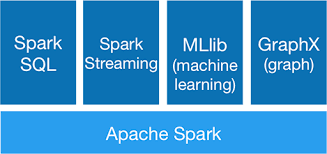
\includegraphics[width=\textwidth]{images/spark.png}
	\caption{Infrastruttura Spark.}
	\label{fig:sparkOverview}
\end{figure}
Nel sistema distribuito, poichè c'è l'esigenza di recuperare i dati in real time dalla coda di bitcoind, viene utilizzato Spark Streaming. Questo modulo è un'estensione dell'API Spark di base che consente l'elaborazione streaming, scalabile, ad alto throughput e con tolleranza agli errori dei flussi di dati in tempo reale. I dati, che possono provenire da diverse fonti, sono elaborati utilizzando algoritmi complessi espressi con funzioni di alto livello come \textit{map}, \textit{reduce}, \textit{join} e \textit{window}. I dati processati, infine possono essere inviati a filesystem (Hadoop) o database (Neo4j) per il salvataggio oppure ad altri moduli di Spark, dediti all'analisi, tipo machine learning (MLlib) o graph processing (GraphX). 
\\Internamente, Spark Streaming riceve streams di dati di input e li divide in batch, che vengono quindi elaborati dal motore Spark per generare il flusso finale di risultati. Per consentire il facile utilizzo di questi dati, fornisce un'astrazione di alto livello chiamata stream discretizzato o DStream, che rappresenta un flusso continuo di dati. E' possibile creare Dstreams da flussi di dati di input da sorgenti come Kafka, Flume e Kinesis o applicando operazioni di alto livello su altri Dstreams \cite{spark:home-streaming}. Internamente, un Dstream è rappresentato come una sequenza di RDD sulla quale possono essere effettuate le operazioni descritte in precedenza.
\begin{figure}[H]
	\centering
	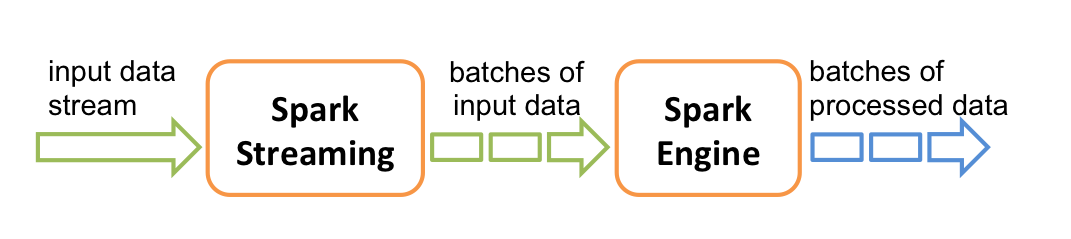
\includegraphics[width=\textwidth]{images/streamingSpark.png}
	\caption{Come vengono gestiti i dati in Spark Streaming.}
	\label{fig:streamingSpark}
\end{figure}

Nel sistema distribuito, per fare analisi dei dati provenienti dall'elaborazione di Spark, è stato scelto il modulo interno Graphx.


\subsection{Hadoop HDFS}
\label{sec:hadoop HDFS}

\subsection{Neo4j}
\label{sec:neo4j}


